\begin{figure*}[t]
    \centering
    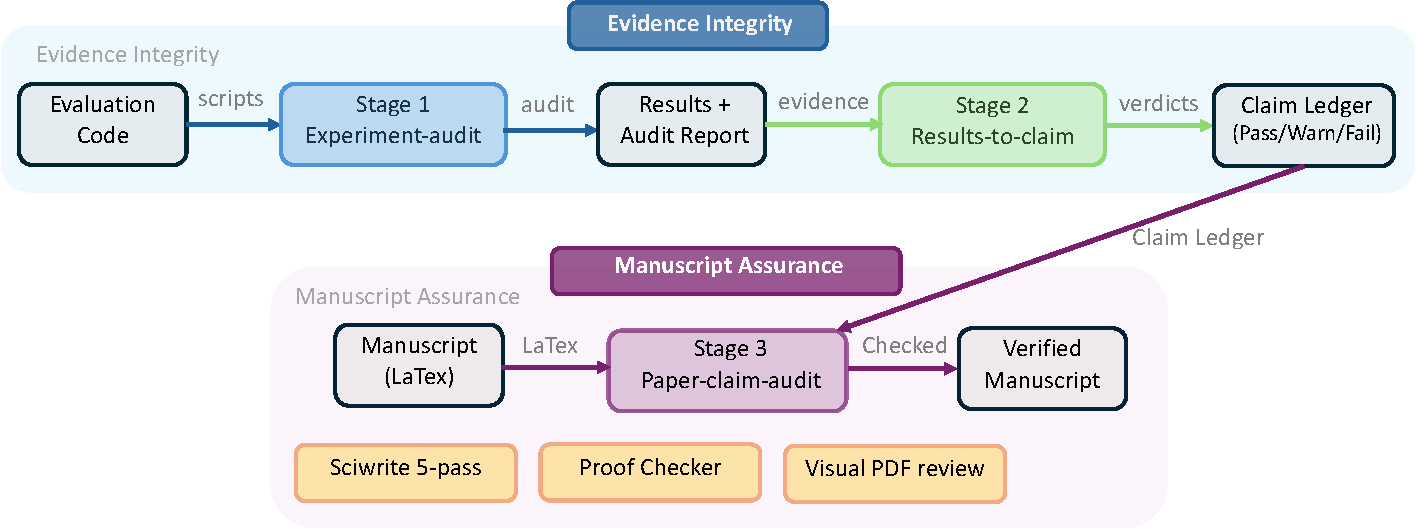
\includegraphics[width=0.95\textwidth]{figures/srcs/03_audit.pdf}
    \caption{Evidence-to-Claim Audit Cascade. \textbf{Stage~1} (\texttt{experiment-audit}): the reviewer audits evaluation scripts and result files for integrity failure modes. \textbf{Stage~2} (\texttt{result-to-claim}): results are mapped to explicit claim verdicts (supported, partial, invalidated); claims with audit failures are downgraded. \textbf{Stage~3} (\texttt{paper-claim-audit}): a zero-context fresh reviewer compares every quantitative claim in the manuscript against the claim ledger and raw result files. The \textbf{Manuscript Assurance} layer applies four components: a five-pass editing pipeline, proof verification, visual PDF review, and citation-audit (verifying every \texttt{\textbackslash cite} for existence, metadata correctness, and context appropriateness).}
    \label{fig:audit}
\end{figure*}
